\section{Сравнение особенностей конструкций с аналогами}
\label{sec:analogs}
Входе изучения существующих решений, аналога рассматриваемой системы, на момент написания курсовой работы, не было обнаружено. Однако ниже приведено сравнение с, так называемыми \textit{sending-cards} -- используется для преобразования входящего видеосигнала в сигнал для \textit{recieving-card}, к которым уже подключаются субмодули.

\subsection{NovaStar MSD600}
\subsubsection{Функционал}
Используется как подключаемое по PCI. В системе определяется, как видеовоспроизводящее решение, имеет четыре порта вывода \textit{RJ-45}. 
\subsubsection{Особенности эксплуатации}
Не функционирует как отдельное устройство. Для работы необходим компьютер, нет возможности подключить напрямую субмодуль.
\begin{figure}[ht]
    \centering
    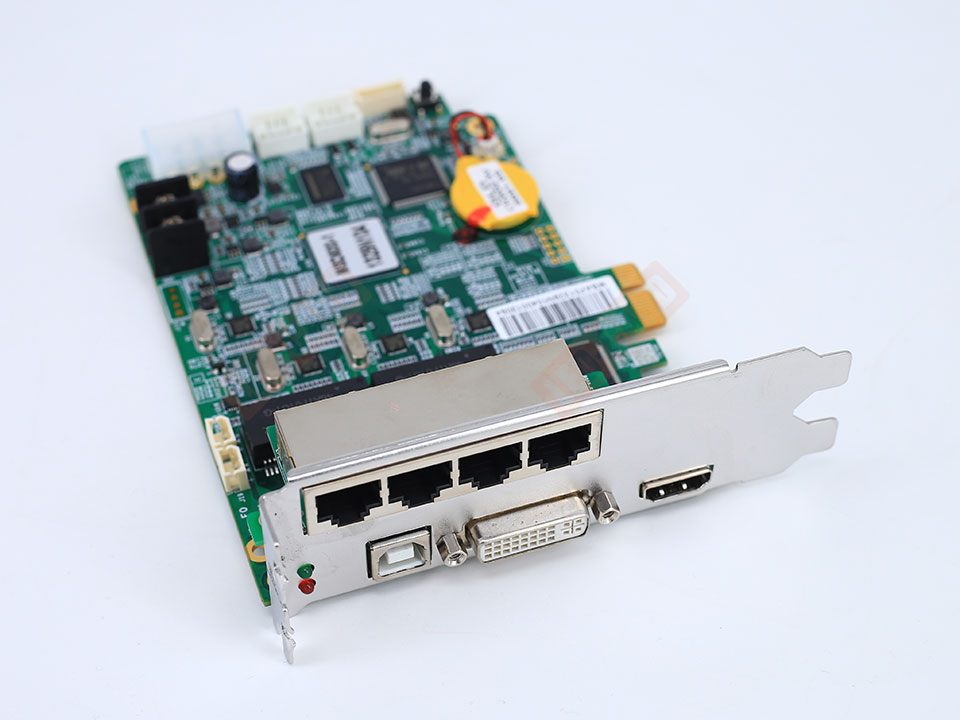
\includegraphics[width=0.6\linewidth]{\commonSecPathPrefix/sec_2/content/Novastar_MSD600.jpg}
    \caption{Novastar MSD600}
\end{figure}
\subsubsection{Сферы применения}
Инсталяции с использованием светодиодных экранов мелкого/среднего размера.
\subsubsection{Стоимость}
На момент написания курсовой работы, стоимость устройства в РБ составляет \(935BYN\).

\subsection{Linsn TS801}
\subsubsection{Функционал}
Используется как подключаемое по PCI. В системе определяется, как видеовоспроизводящее решение, имеет два порта вывода \textit{RJ-45}. 
\subsubsection{Особенности эксплуатации}
Не функционирует как отдельное устройство. Для работы необходим компьютер, нет возможности подключить напрямую субмодуль.
\begin{figure}[ht]
    \centering
    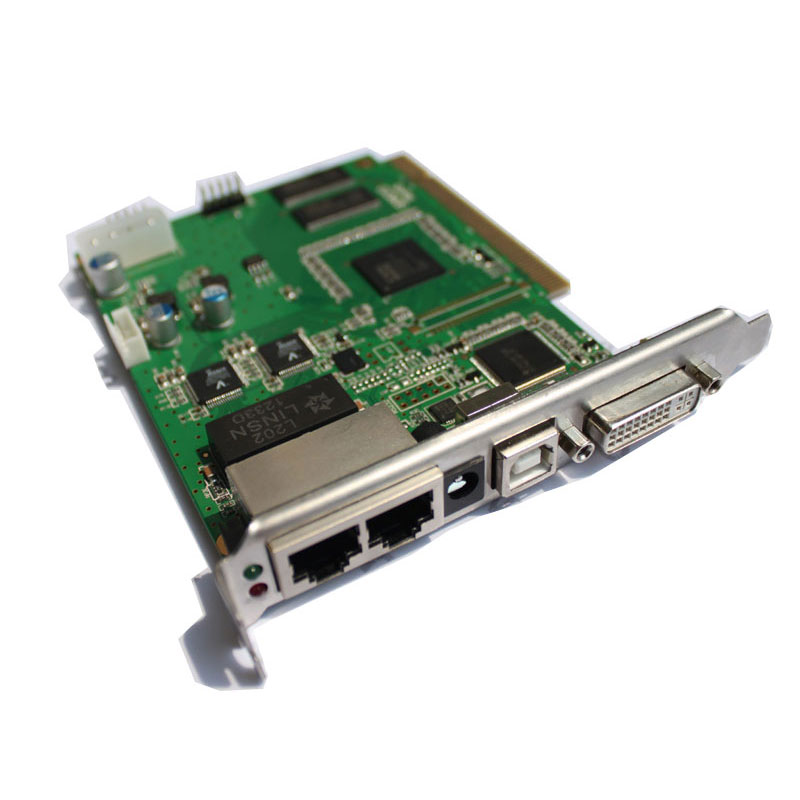
\includegraphics[width=0.6\linewidth]{\commonSecPathPrefix/sec_2/content/linsn-ts801d.jpg}
    \caption{Novastar MSD600}
\end{figure}
\subsubsection{Сферы применения}
Небольшие инсталяции светодиодных экранов.
\subsubsection{Стоимость}
На момент написания курсовой работы, стоимость устройства в РБ составляет \(621BYN\).

\subsection{Novastar H9}
\subsubsection{Функционал}
\begin{figure}[ht]
    \centering
    \includegraphics[width=0.6\linewidth]{\commonSecPathPrefix/sec_2/content/h9.png}
    \caption{Novastar MSD600}
\end{figure}
\subsubsection{Особенности эксплуатации}
Высокое энергопотребление.
\subsubsection{Сферы применения}
Устройство является мощным инструментом для подключения большого количества модулей светодиодного экрана. Применяется в местах, где необходимо обеспечить отказоустойчивое подключение экранов.
\subsubsection{Стоимость}
На момент написания курсовой работы, стоимость устройства в РБ составляет \(1072BYN\).
